\documentclass[10pt]{article}
\usepackage[russian]{babel}
\usepackage[utf8]{inputenc}
\usepackage{amssymb}
\usepackage{amsmath}
\usepackage{latexsym}
\usepackage{enumitem}
\usepackage[margin=2cm]{geometry}
\usepackage{tikz}
\usepackage{graphicx}
\usetikzlibrary{arrows}

\begin{document}

\title{Домашняя работа 2}
\author{Антон Афанасьев}
\maketitle

\begin{enumerate}

\item[2.9] Будем строить неориентированное дерево следующим образом: возьмем вершину орграфа с входящей степенью 0. Добавим исходящее из нее ребро в дерево (соединим вершины с такими же номерами в дереве ребром) и удалим эту вершину с ребром. Будем продолжать, пока можем. Такие действия не нарушают дерева, так как, если при добавлении ребра в дерево образовался цикл, то это значит, что либо где-то раньше была вершина с исходящей степенью больше одного (а такого нет по условию), либо мы пытаемся пойти в одну из уже удаленных вершин.\\
После таких действий у нас в орграфе останется некоторое количество не пересекающихся циклов (пересекаться они не могут, т.к. исходящая степень каждой вершины один). А в недоделанном дереве будет лес, причем вершины, лежащие на оставшихся циклах, вершины 1 и $n$, находятся в разных компонентах связности (на них заканчивалось построение компоненты связности).\\
Теперь посмотрим на не пересекающиеся циклы как на перестановку и запишем ее в явном виде как последовательность номеров вершин. $i$-тый элемент последовательности --- номер вершины в который переходит под действием перестановки $i$-тая по возрастанию вершина из множества оставшихся. Теперь соединим эти вершины ребрами в дереве в порядке перестановки начиная с 1 и заканчивая $n$ (запишем перестановку ``между ними''). Таким образом мы соединим все компоненты связности и получим дерево на $n$ вершинах.\\
По любому дереву можно однозначно восстановить орграф заданного вида обратными действиями. Будем теперь от дерева откусывать по листу, если этот лист не 1 и не $n$ и добавлять направленное ребро от листа к его соседу в орграф. После таких операций останутся только вершины 1, $n$ и, возможно, какие-то вершины между ними. Выпишем эти вершины в порядке обхода от 1 до $n$ и посмотрим на них, как на перестановку. Добавим оставшиеся ребра и получим нужный орграф.

\item[3.11] Удалим вершины, отмеченные на рисунке\\
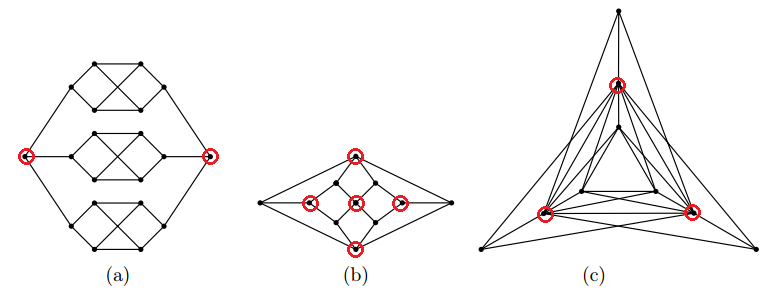
\includegraphics[width=\textwidth]{3_11.png}
Во всех случаях поле удаления вершин граф распадается на на компоненты связности, число которых больше чем число удаленных вершин.

\item[3.12] Граф Петерсена не является гамильтоновым.\\
Рассмотрим граф Петерсена в таком виде:
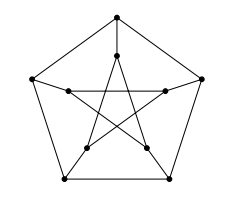
\includegraphics{petersen.png}\\
Предположим, что гамильтонов цикл существует. Тогда он должен когда-то войти в ``звезду'', а потом выйти из нее, возможно несколько раз. Он мог зайти и выйти в звезду либо один, либо два раза(три уже не мог, так как в звезде 5 вершин). Будем считать, что ``начало'' цикла находится на ``окружности'', а следующая вершина в цикле --- соответствующая вершина на ``звезде''.\\
Предположим, что цикл заходит в ``звезду'' и выходит из нее один раз. Но путь, начинающийся из какой-либо вершины звезды, и обходящий ее всю, заканчивается в одной из ``противоположных'' вершин и никогда не заканчивается в ``соседних''. Это означает, что оставшаяся окружность оказывается разделена на две части, которые нельзя обойти не заходя в вершину из которой мы начали дважды. Поэтому гамильтонова цикла не получится.\\
Предположим, что цикл заходит в ``звезду'' и выходит из нее дважды. Так как в ней 5 вершин, это означает, что один в раз мы должны посетить 3 вершины (будем считать этот раз первым. по предположению у нас цикл, так что нам все равно), а в другой оставшиеся две. После первого захода в ``звезду'' мы выйдем в вершине ``соседней'' с той, из которой мы начали. После этого будем двигаться по окружности в сторону не посещенных вершин (это единственный способ все-таки их посетить). Зайти в ``звезду'' второй раз у нас есть два способа, либо в следующей вершине окружности, либо через две. Если мы заходим в звезду в следующей вершине, то после выхода из звезды останется одна не посещенная вершина на окружности, и мы не сможем замкнуть цикл. Если мы заходим в звезду из дальней от нас вершины окружности, то мы закончим в вершине ``звезды'' и тоже не сможем замкнуть цикл.\\
Таким образом, в этом графе циклов нет.\\

\item[3.14] Можно:\\
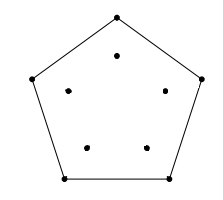
\includegraphics{3_14.png}\\
Если добавить ограничение, на то, что оставшийся граф должен быть связным, то получается, что для каждой вершины мы должны удалить одно инцидентное ребро (чтобы сделать у каждой вершины степень 2). Для каждой вершины на ``окружности'' мы должны решить оставлять у нее ребро в ``звезду'' или нет. Убрать ребро в звезду, так чтобы у остальных вершин на окружности была степень 2, можно у одной, трех или пяти вершин. Теперь если выкидывать ребра из ``звезды'' так, чтобы у них этих вершин была степень два, то получится, что в случае с одной и пятью вершинами граф не связный, а для случая с 3 вершинами нельзя добиться степени 2 у вершин звезды. Значит, в нельзя убрать ребра в графе Петерсена так, чтобы граф остался связным и в нем существовал эйлеров цикл.\\
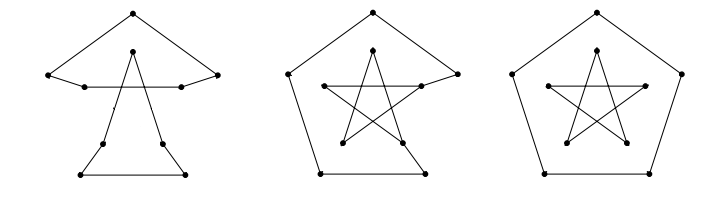
\includegraphics{3_14_2.png}
\end{enumerate}

\end{document}
